\documentclass[10pt]{beamer}

\usetheme{default}

\usepackage[utf8]{inputenc}
\usepackage[russian]{babel}
\usepackage[OT1]{fontenc}
\usepackage{amsmath}
\usepackage{amsfonts}
\usepackage{amssymb}
\usepackage{graphicx}
\usepackage{etoolbox}
\usepackage{caption}
\usepackage{subcaption}
\usepackage{pifont}
\usepackage{xcolor}
\usepackage{framed}
\definecolor{shadecolor}{cmyk}{0,0,0,1}
\usepackage{listings}

\lstset{
    backgroundcolor=\color{lightgray},
    commentstyle=\color{blue},
    frame=single
    breakatwhitespace, 
    language=python, 
    columns=fullflexible, 
    keepspaces, 
    breaklines, 
    tabsize=3, 
    subfigurehowstringspaces=false, 
    extendedchars=true,
    numbers=left
}

\makeatletter

\setbeamercolor{title}{fg=white}
\setbeamercolor{frametitle}{fg=black}
\setbeamerfont*{title}{family=\sffamily,size=\LARGE}

\setbeamerfont{page number in head/foot}{size=\scriptsize}
\setbeamertemplate{footline}[frame number]
\let\otp\titlepage
\renewcommand{\titlepage}{\otp\addtocounter{framenumber}{-1}}

\setbeamertemplate{background canvas}{%
	\ifnumequal{\c@framenumber}{0}{%
      
\includegraphics[width=\paperwidth,height=\paperheight]{images/cover.png}
   }{%
      \ifnumequal{\c@framenumber}{\inserttotalframenumber}{
         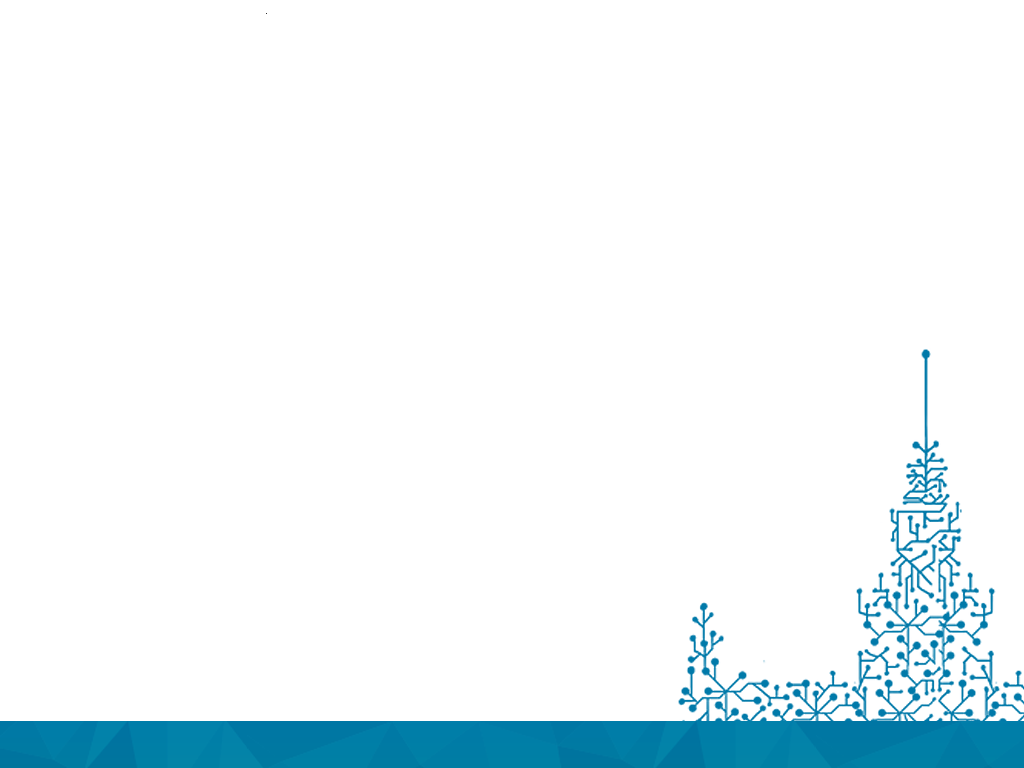
\includegraphics[width=\paperwidth,height=\paperheight]{images/back.png}
      }{%
         % Other frames
      }%
   }%
}

\makeatother

\beamertemplatenavigationsymbolsempty

\author{Владимир Гулин}
\title{\newline \newline \newline Лекция 9 \\ Алгоритмические композиции\\
Начало}

\begin{document}

\defverbatim[colored]\bagging{%
\begin{lstlisting}[tabsize=4,basicstyle=\ttfamily]
function BaggingRSM(X, F, poi, pof, T):
    # X - point from dataset
    # F - original set of features
    # poi - percent of items
    # pof - percent of features
    # T - number of algorithms
    for j in 1..T:
        fsubset = sample_features(F, pof)
        xsubset = sample_items(X, poi) 
        a_j = build_base_model(xsubset, fsubset)
 
    return a_1 ... a_T
\end{lstlisting}
}

\begin{frame}[plain]
\titlepage
\end{frame}

\begin{frame}{План лекции}
\tableofcontents
\end{frame}

% =======================
\section{Мотивация}
% =======================

\begin{frame}{Выбираем ноутбук}

\begin{columns}[C]
        \centering
        \begin{column}{.5\textwidth}
                \begin{block}{Параметры ноутбука}
                \begin{itemize}
                    \item Камень
                    \item Память
                    \item Видеокарта
                    \item Диагональ монитора
                    \item и т.д
                \end{itemize}
                \end{block}
        \end{column}%        
        \begin{column}{.5\textwidth}
                \begin{center}
                    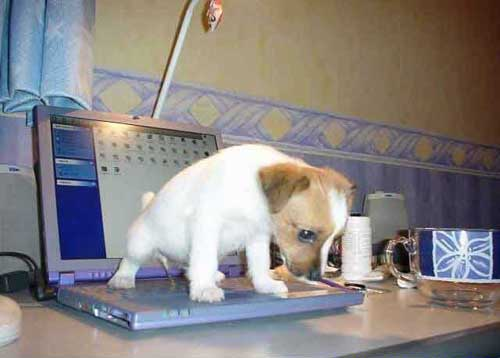
\includegraphics[scale=0.3]{images/book.jpg}
                \end{center}
        \end{column}
\end{columns}

\begin{block}{Воспользуемся экспертным мнением}
\begin{itemize}
    \item Консультант в магазине
    \item Сосед ``программист''
    \item Друзья
    \item Форумы
\end{itemize}
\end{block}

\end{frame}

\begin{frame}{Задача обучения с учителем}
\begin{block}{Постановка задачи}
\end{block}

Пусть дан набор объектов $\mathcal{D} = \{(\mathbf{x}_i, y_i)\},
\; \mathbf{x}_i \in \mathcal{X},
\; y_i \in \mathcal{Y},
\; i \in 1, \ldots, N$, полученный из неизвестной закономерности $y =
f(\mathbf{x})$. Необходимо построить такую $h(\mathbf{x})$, которая наиболее точно
апроксимирует $f(\mathbf{x})$.

\vspace{1em}
Будем искать неизвестную 
\[
    h(\mathbf{x}) = C(a_1(\mathbf{x}), \ldots, a_T(\mathbf{x}))
\]

$a_i(\mathbf{x}):\mathcal{X} \rightarrow \mathcal{R}, \,\, \forall i \in
\{1,\ldots, T\}$ - базовые модели 

$C: \mathcal{R} \rightarrow \mathcal{Y}$ - решающее правило
\end{frame}

% =======================
\section{Обзор методов построения алгоритмических композиций}
% =======================

\begin{frame}{Простое голосование}
\begin{block}{Simple Voting}
\end{block}
\[
    h(\mathbf{x}) = \frac{1}{T} \sum \limits_{i=1}^{T} a_i(\mathbf{x})
\]
\begin{center}
    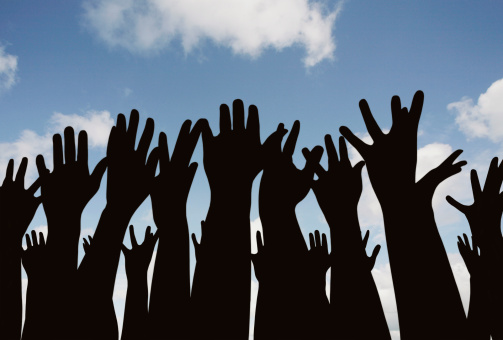
\includegraphics[scale=0.3]{images/voting.jpg}
\end{center}

\end{frame}

\begin{frame}{Взвешенное голосование}
\begin{block}{Weighted Voting}
\end{block}
\[
    h(\mathbf{x}) = \frac{1}{T} \sum \limits_{i=1}^{T}b_i a_i(\mathbf{x}), \,\,
    b_i \in \mathcal{R}
\]
\begin{center}
    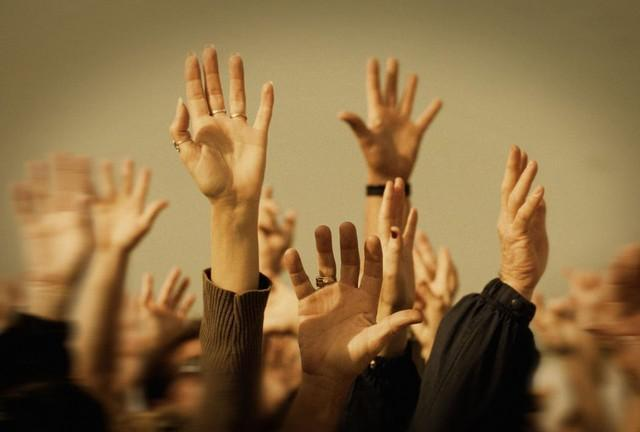
\includegraphics[scale=0.6]{images/wvoting.jpg}
\end{center}

\end{frame}

\begin{frame}{Смесь экспертов}
\begin{block}{Mixture of Experts}
\end{block}
\[
    h(\mathbf{x}) = \frac{1}{T} \sum \limits_{i=1}^{T}b_i(\mathbf{x}) a_i(\mathbf{x}), \,\,
    b_i(\mathbf{x}): \mathcal{X} \rightarrow \mathcal{R}
\]
\begin{center}
    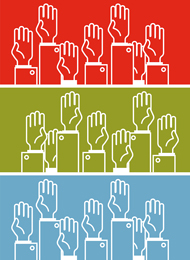
\includegraphics[scale=0.6]{images/mixtureofexperts.jpg}
\end{center}
\end{frame}

\begin{frame}{Топологические композиции}
\begin{block}{Модельные деревья решений (Model decision trees)}
\end{block}
\begin{itemize}
    \item Поместим в листья деревьев какие-нибудь алгоритмы вместо констант
\end{itemize}
\begin{center}
    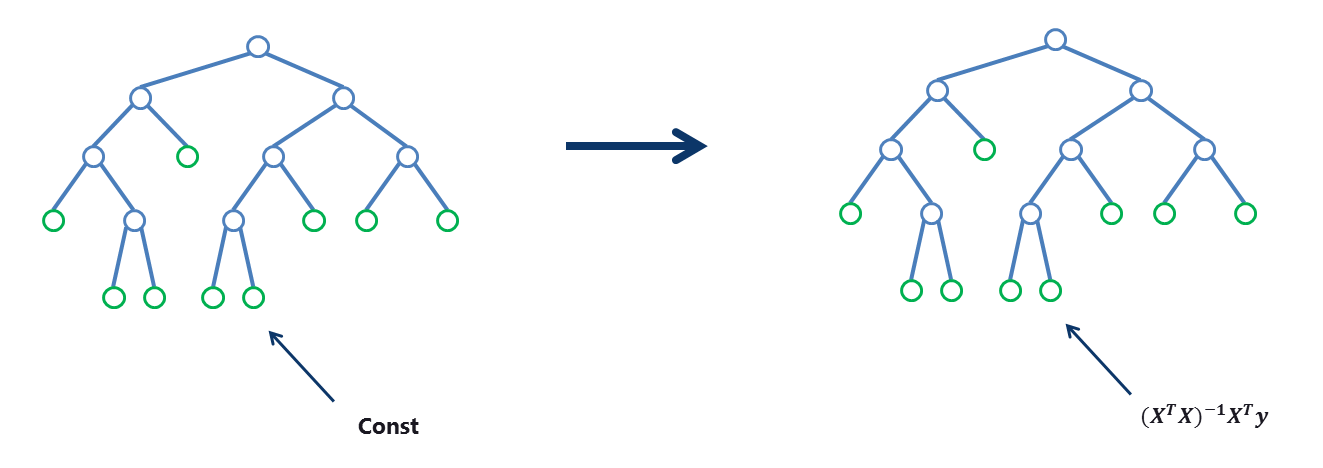
\includegraphics[scale=0.25]{images/modeldt.png}
\end{center}
\end{frame}

\begin{frame}{Нейронные сети}
\begin{block}{Neural networks}
\end{block}
\begin{center}
    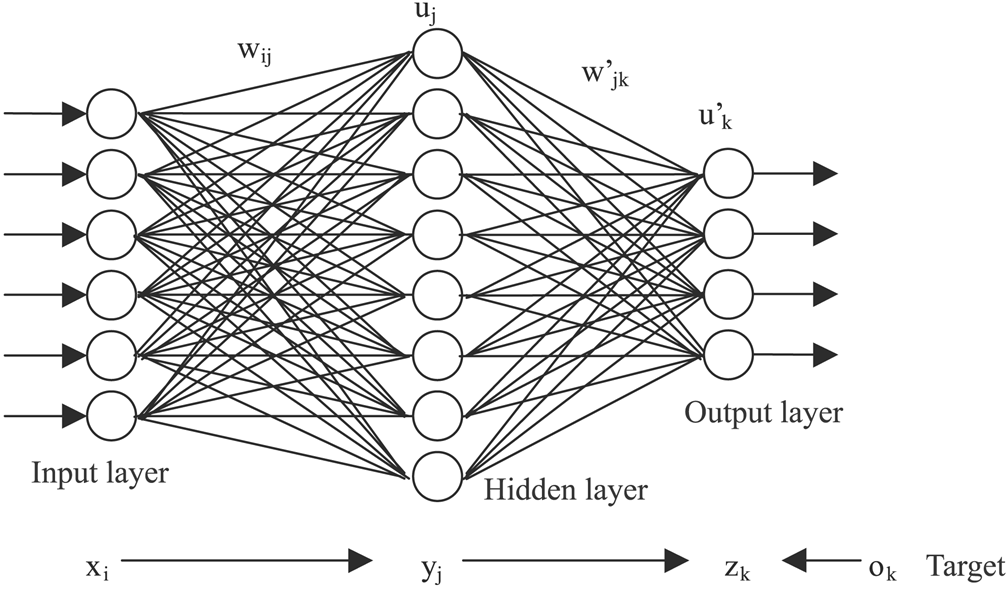
\includegraphics[scale=0.2]{images/NeuralNetwork.png}
\end{center}
    $h(\mathbf{x}) = g(\mathbf{w}^T \mathbf{x})$ - композиция линейных моделей
\end{frame}

\begin{frame}{Текущее положение дел}
\begin{center}
\begin{block}{Decision Trees Compositions vs Neural Nets}
\end{block}
    
\includegraphics[scale=0.4]{images/termvsrobo.jpg}
\end{center}
\end{frame}

\begin{frame}{Neural nets}
\begin{center}
\begin{block}{Где нейронные сети побеждают?}
\begin{itemize}
    \item Computer Vision (ImageNet)
    \item Speech recognition
\end{itemize}
\end{block}
    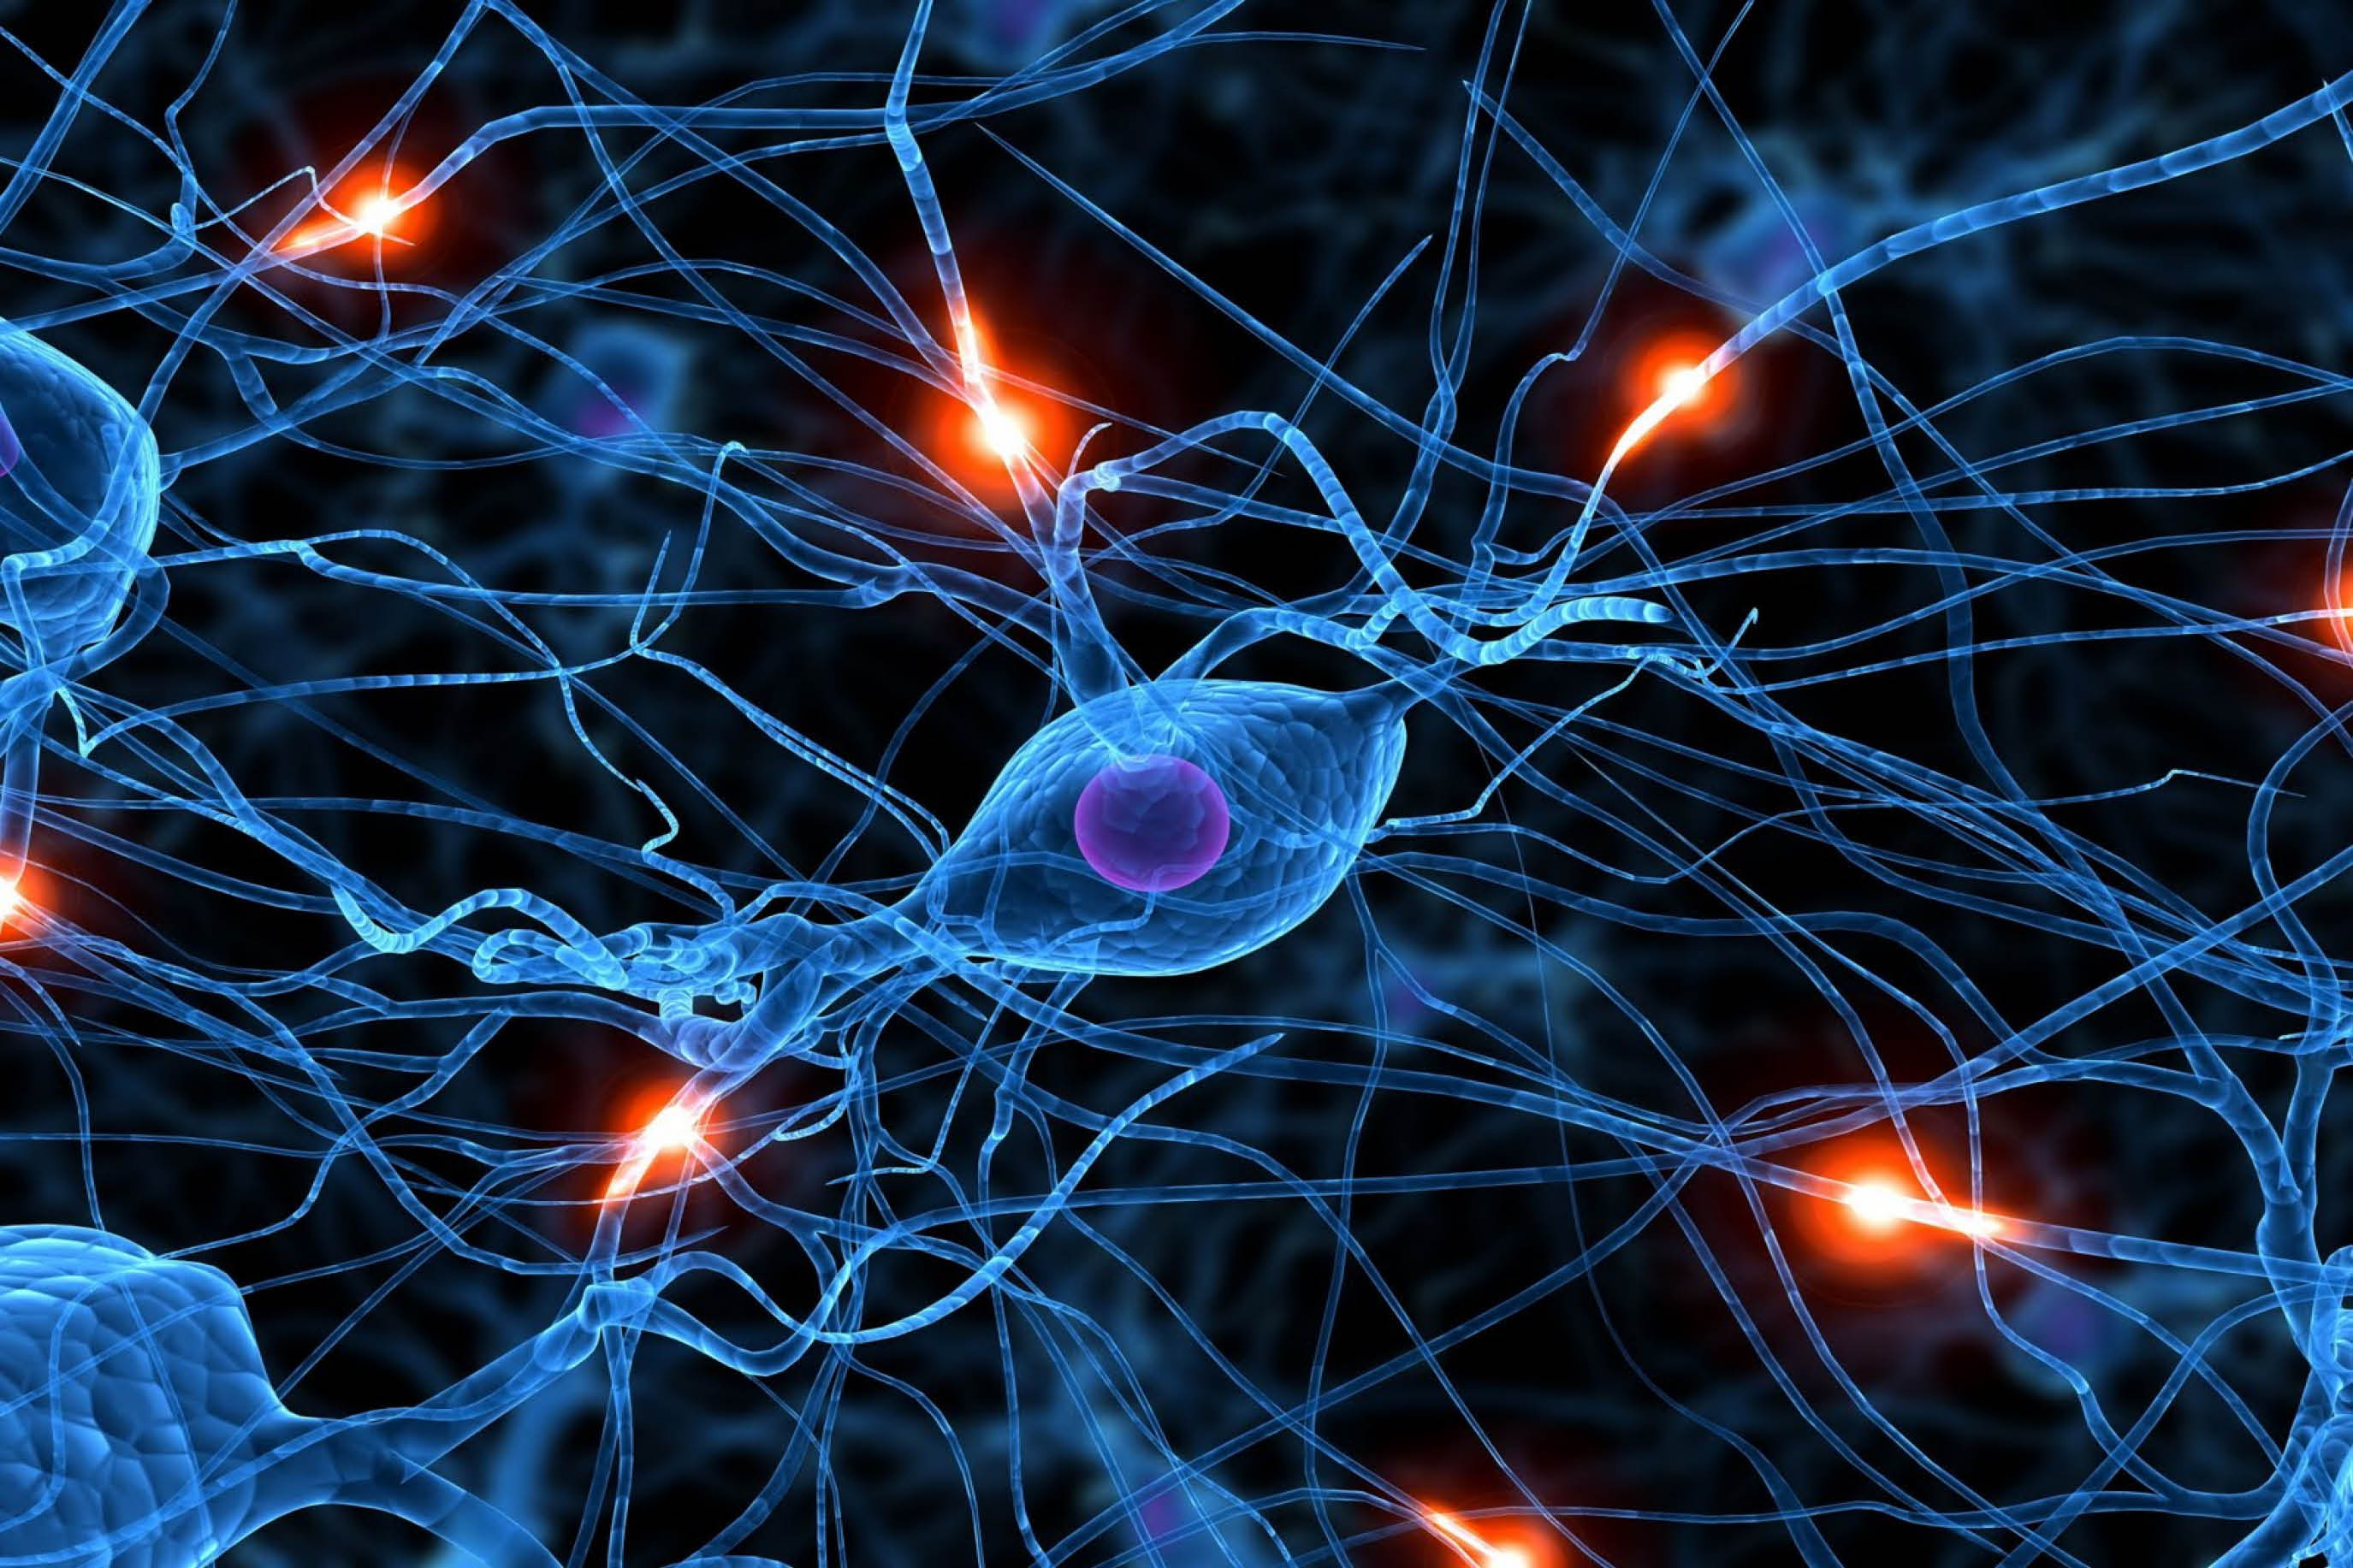
\includegraphics[scale=0.3]{images/nn.jpg}
\end{center}
\end{frame}

\begin{frame}{Decision trees compositions}
\begin{center}
\begin{block}{Где побеждают ансамбли деревьев решений?}
\begin{itemize}
    \item Learning to rank (Yahoo Learning to rank challenge 2010)
    \item Text categorization (NIPS 2006)
    \item Везде
\end{itemize}
\end{block}
    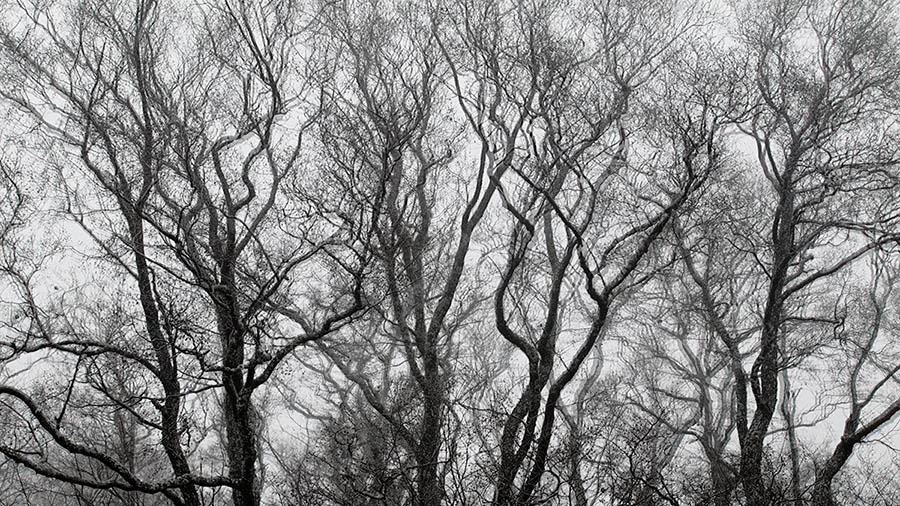
\includegraphics[scale=1.0]{images/forest.jpg}
\end{center}
\end{frame}

\begin{frame}{Взгляд с точки зрения функционального анализа}
\begin{columns}[C]
        \centering
        \begin{column}{.5\textwidth}
                \begin{block}{Гладкие функции}
                \end{block}
                \[
                    h(\mathbf{x}) = \sum \sigma ( \ldots \sum \sigma
                    (\mathbf{w}^T \mathbf{x}) )
                \]
                \begin{center}
                    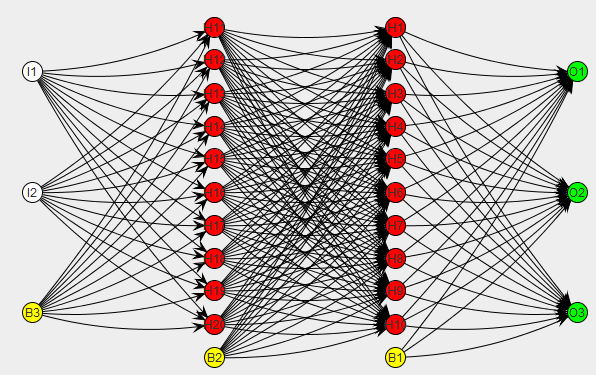
\includegraphics[scale=0.2]{images/nn.png}\\
                    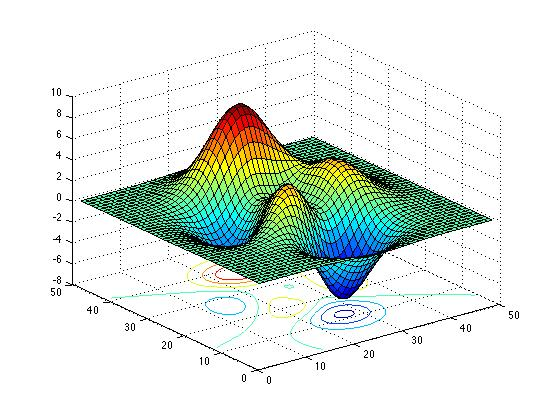
\includegraphics[scale=0.2]{images/nnsurface.jpg}
                \end{center}
        \end{column}%        
        \begin{column}{.5\textwidth}
                \begin{block}{Кусочно-постоянные функции}
                \end{block}
                \[
                    h(\mathbf{x}) = \sum \limits_d c_d  I\{\mathbf{x} \in R_d\}
                \]
                \begin{center}
                    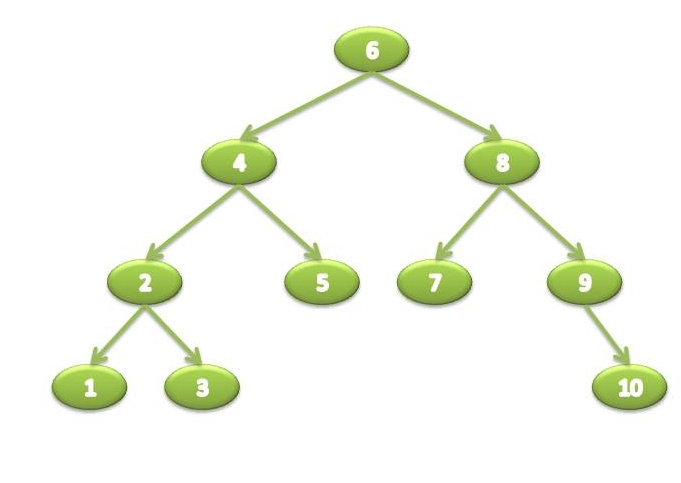
\includegraphics[scale=0.2]{images/tree.jpg}\\
                    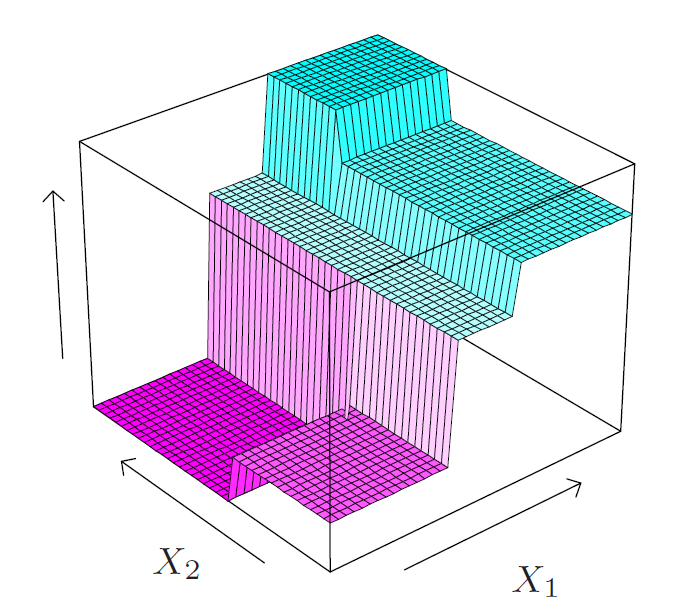
\includegraphics[scale=0.1]{images/treesurface.png}
                \end{center}
        \end{column}
\end{columns}
\end{frame}

\begin{frame}{Методы построения алгоритмических композиций}
\begin{block}{Стохастические методы}
\end{block}
\begin{block}{Бустинг}
\end{block}
\begin{block}{Мета алгоритмы. Stacking}
\end{block}
\end{frame}

\begin{frame}{Stacking}
\begin{block}{Мета-алгоритм}
\end{block}
\begin{center}
    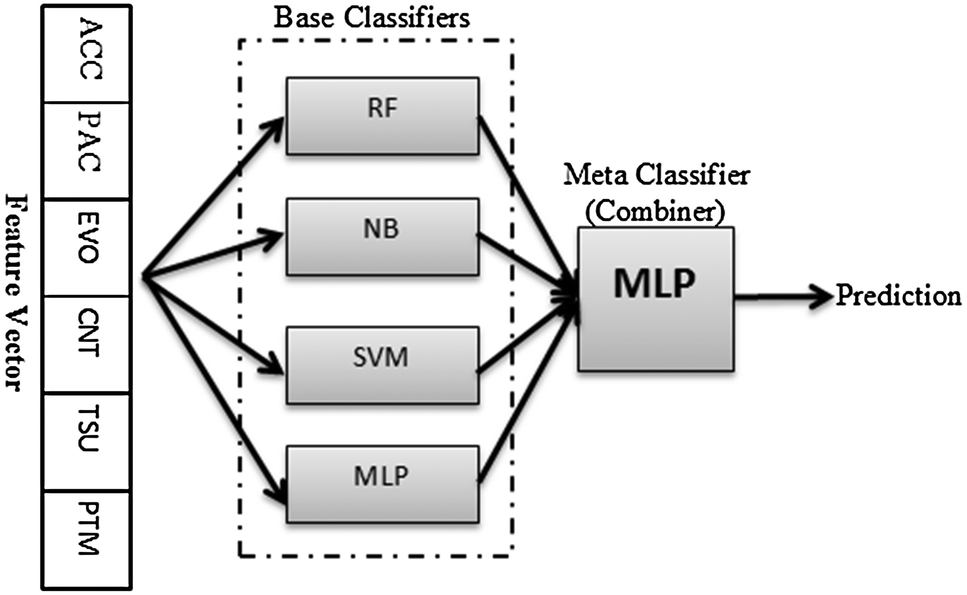
\includegraphics[scale=0.3]{images/stacking.png}
\end{center}
\end{frame}

\begin{frame}{Netflix Challenge}
\begin{center}
    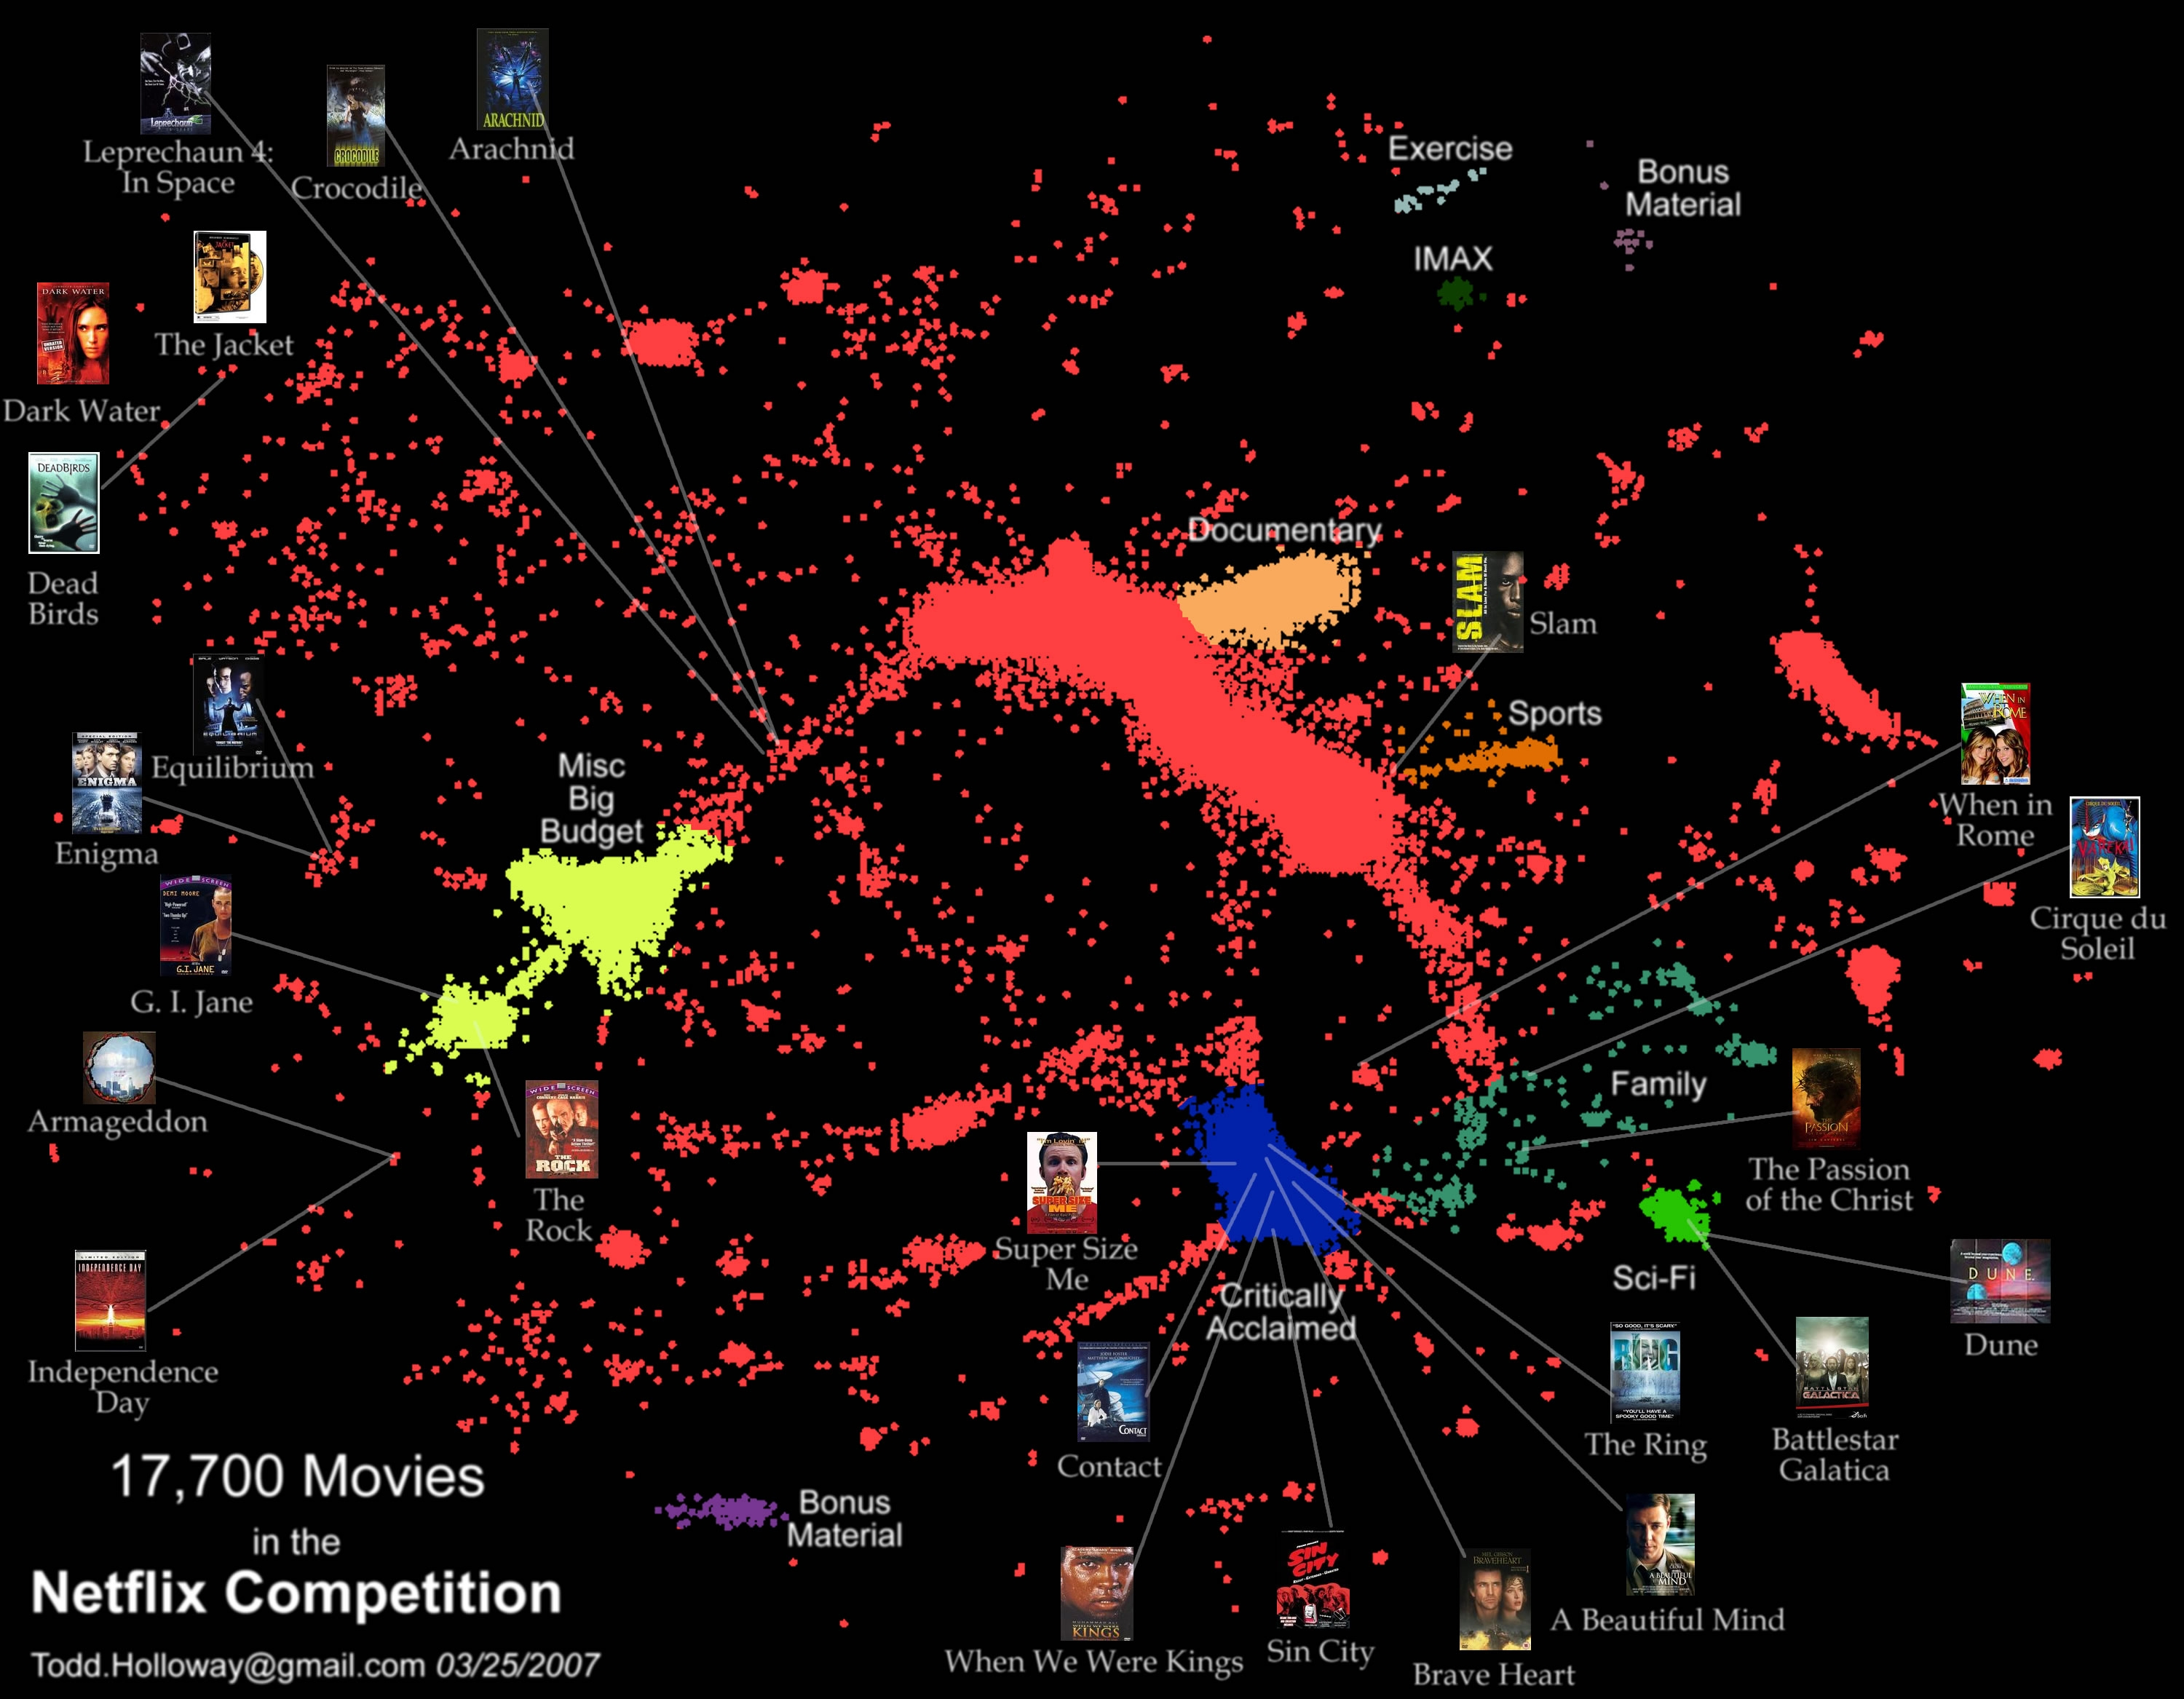
\includegraphics[scale=0.05]{images/netflix.jpg}
\end{center}
\begin{itemize}
    \item Задача предсказания оценки фильму
    \item ПФ - 1000000\$
    \item Победил Stacking на ``зоопарке'' алгоритмов
\end{itemize}
\end{frame}

\begin{frame}{Немного теории}
    \begin{center}
        
\includegraphics[scale=0.2]{images/houseprice.png}\\
        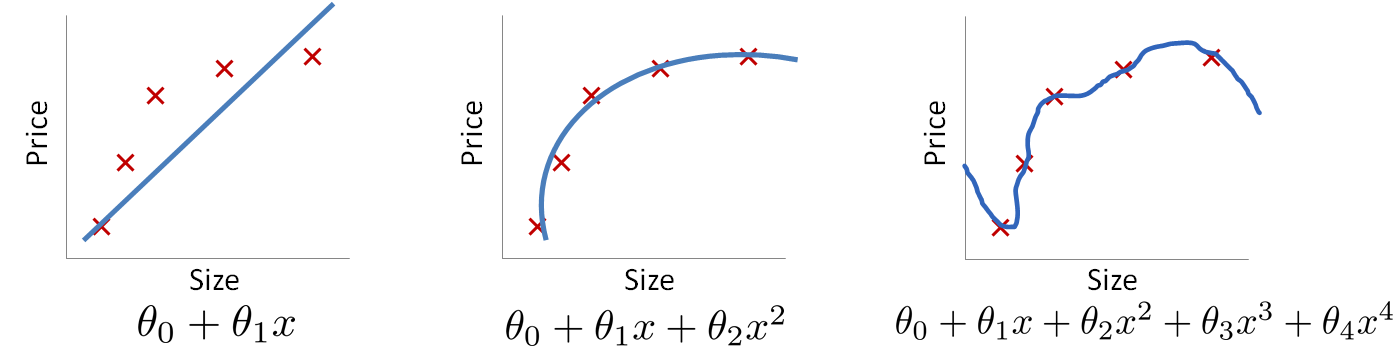
\includegraphics[scale=0.2]{images/linreg.png}
    \end{center}
\textbf{Недообучение} - сложность модели недостаточна. Данные имеют более
сложную природу.

\textbf{Переобучение} - сложность модели избыточна. Модель слишком настроена на
выборку. Обобщающая способность алгоритма низка.
\end{frame}

\begin{frame}{The bias-variance Decomposition}
\begin{itemize}
    \item Задача регресии
    \item $y=f(x) + \epsilon$
    \item $\epsilon \sim \mathcal{N}(0, \sigma_{\epsilon})$
    \item Ищем $h(\mathbf{x})$ аппроксимирующую $f(\mathbf{x})$
Таким образом, мы можем оценить ожидание среднеквадратичной ошибки для
некоторой точки $\mathbf{x}_0$
\end{itemize}
\[
    Err(\mathbf{x}_0) = E[(y - h(\mathbf{x}_0))^2]
\]
Это можно переписать в виде
\[
    Err(\mathbf{x}_0) = (E[h(\mathbf{x}_0)] - f(\mathbf{x}_0))^2 +
    E[h(\mathbf{x}_0) - E(h(\mathbf{x}_0))]^2 + \sigma_{\epsilon}^2
\]
\[
    Err(\mathbf{x}_0) = Bias^2 + Variance + Noise (Irreducible\,\, Error)
\]
\end{frame}

\begin{frame}{Bias and variance tradeoff}
\begin{columns}[C]
    \centering
    \begin{column}{.45\textwidth}
        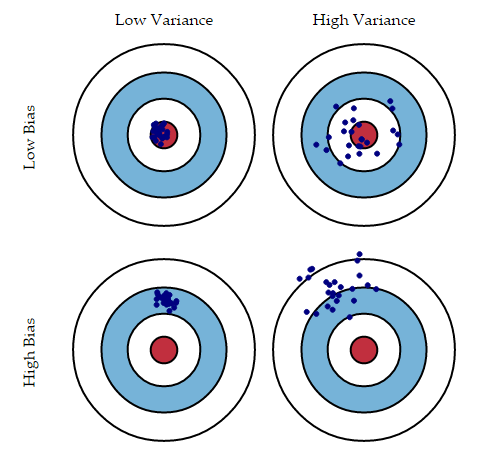
\includegraphics[scale=0.35]{images/biasandvariance.png}
    \end{column}
    \begin{column}{.45\textwidth}
        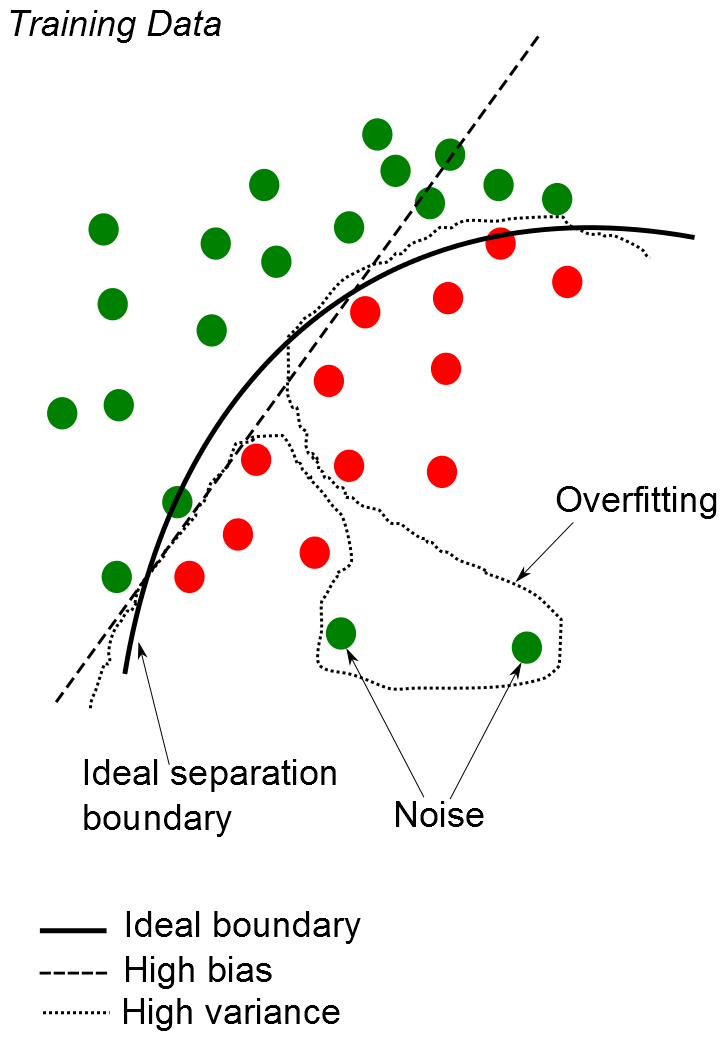
\includegraphics[scale=0.2]{images/bias_variance.png}
    \end{column}
\end{columns}
\end{frame}

\begin{frame}{Bias and variance tradeoff}
    \begin{center}
        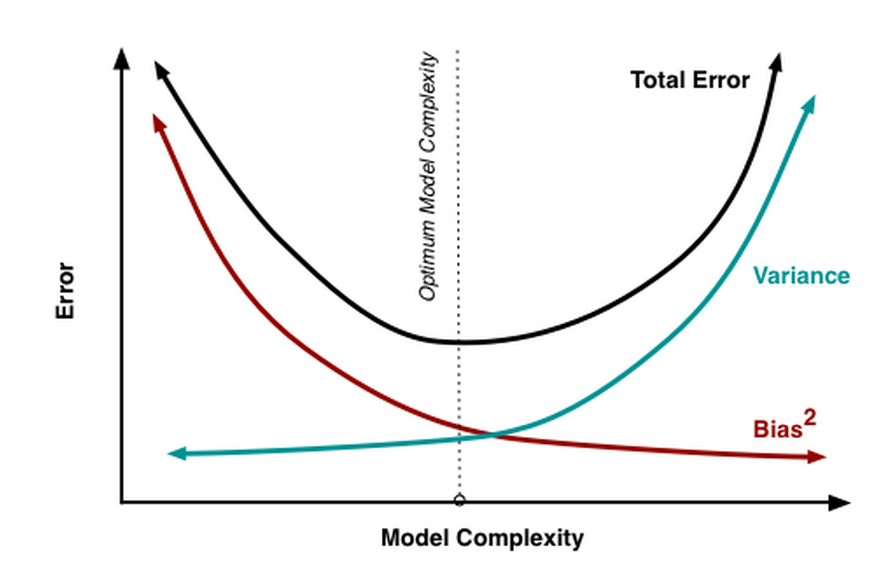
\includegraphics[scale=0.3]{images/learningcurves.png}
    \end{center}
\end{frame}

% =======================
\section{Стохастические методы построения алгоритмических композиций}
% =======================

\begin{frame}{Стохастические методы}
\begin{block}{Стратегии}
\end{block}
\begin{itemize}
    \item \textbf{Bagging = Bootstrap aggregation}. Обучаем алгоритмы по
        случайным подвыборкам размера $N$, полученным с помощью выбора с
        возвращением.
    \item \textbf{RSM = Random Subspace Method}. Метод случайных
        подпространств. Обучаем алгоритмы по случайным подмножествам признаков.
\end{itemize}

\vspace{1em}
Благодаря описанным стратегиям добиваемся максимального различия между базовыми
алгоритмами.
\end{frame}

\begin{frame}{Bagging \& RSM}
\bagging
\end{frame}

\begin{frame}{Bagging \& RSM}
\begin{block}{Геометрическая интерпрeтация}
\end{block}
\begin{center}
    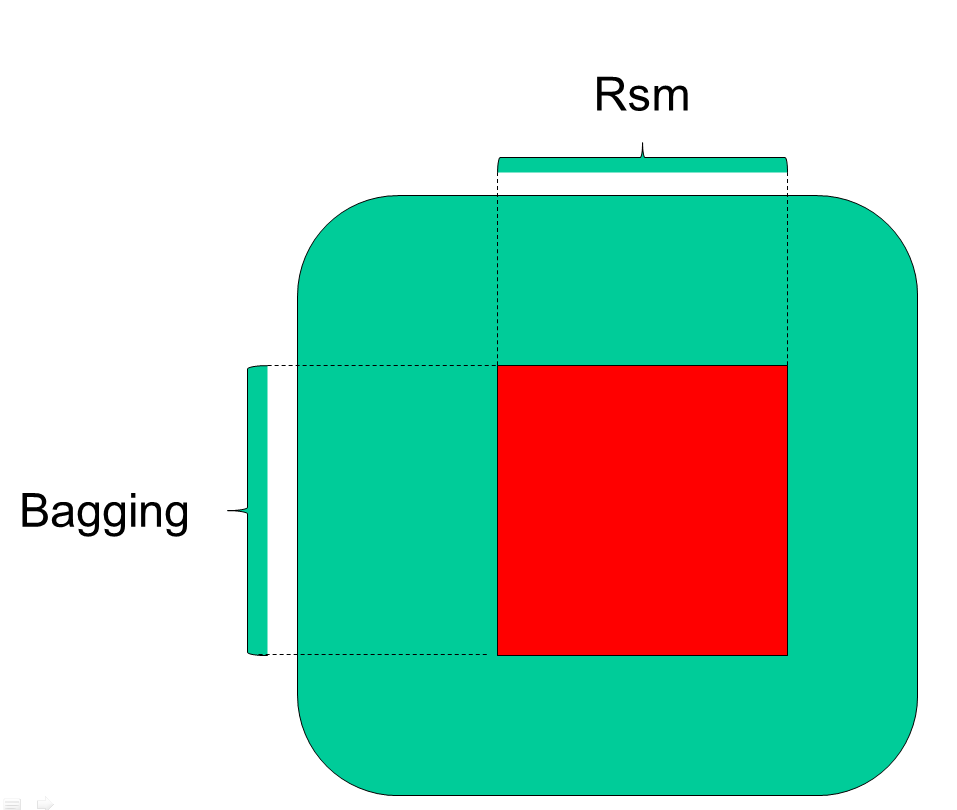
\includegraphics[scale=0.2]{images/baggingandrsm.png}
\end{center}
\end{frame}

\begin{frame}{Bias-Variance for Bagging \& RSM}
Модель простого голосования
\[
    h(\mathbf{x}) = \frac{1}{T} \sum \limits _{i=1}^T a(\mathbf{x})
\]
Смещение и разброс
\[
    Bias^2 = (E[h(\mathbf{x}_0)] - f(\mathbf{x}_0))^2 = (E[a(\mathbf{x}_0)] -
    f(\mathbf{x}_0))^2 
\]
\[
    Variance = E[h(\mathbf{x}_0) - E(h(\mathbf{x}_0))]^2 =
\]
\[
    = \frac{1}{T} \sum
    \limits_{i=1}^T E[a_i(\mathbf{x}_0) - E[a_i(\mathbf{x}_0)]]^2 + 
\]
\[
    +\frac{1}{T} \sum \limits
    _{i \neq j} E[(a_i(\mathbf{x}_0) -
    E[a_i(\mathbf{x}_0)])(a_j(\mathbf{x}_0) - E[a_j(\mathbf{x}_0)])] =
\]
\[
    = \frac{1}{T} \sum \limits_{i=1}^T E[a_i(\mathbf{x}_0) -
    E[a_i(\mathbf{x}_0)]]^2 + \frac{1}{T} \sum \limits _{i \neq j}
    cov(a_i(\mathbf{x}_0), a_j(\mathbf{x}_0))
\]
\end{frame}

% =======================
\section{Random Forest}
% =======================

\begin{frame}{Random Forest}
Случайный лес (random forest) - bagging \& rsm над решающими деревьями.
\begin{center}
    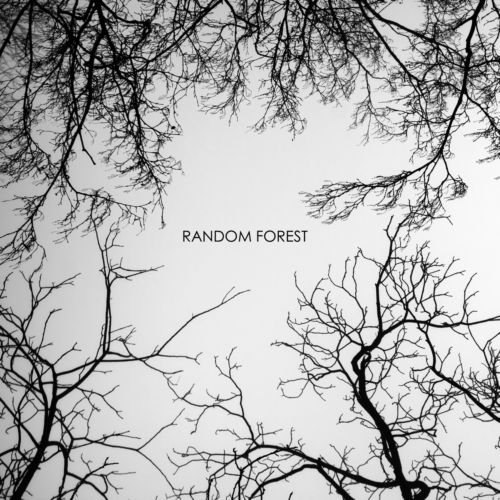
\includegraphics[scale=0.3]{images/rf.jpg}
\end{center}
\end{frame}

\begin{frame}{``Неустойчивость'' деревьев решений}
\begin{itemize}
    \item Незначительные изменения в данных приводят к значительным изменениям в
    топологии дерева
\end{itemize}
\begin{figure}
    \centering
    \begin{subfigure}[b]{0.45\textwidth}
        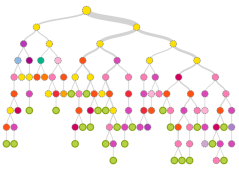
\includegraphics[width=\textwidth]{images/tree1.png}
    \end{subfigure}
    \begin{subfigure}[b]{0.45\textwidth}
        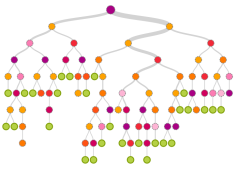
\includegraphics[width=\textwidth]{images/tree2.png}
    \end{subfigure}
\end{figure}
\end{frame}

\begin{frame}{Random Forest. Пример}
\begin{center}
    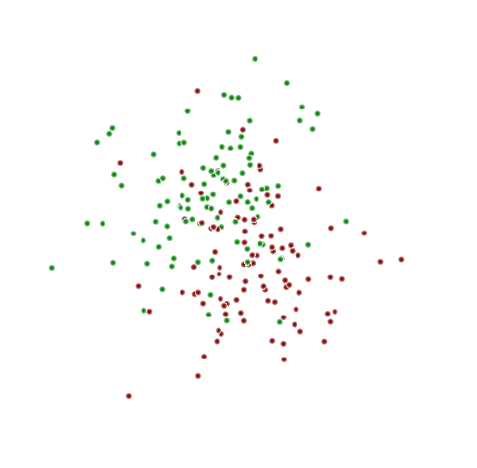
\includegraphics[scale=0.25]{images/rforig.png}
\end{center}
\begin{figure}
    \centering
    \begin{subfigure}[b]{0.3\textwidth}
        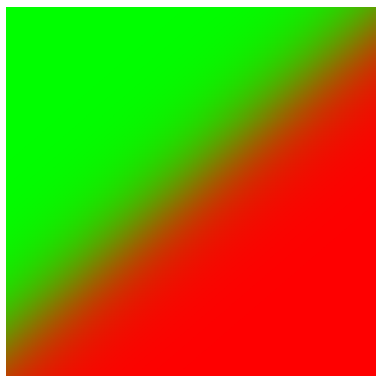
\includegraphics[width=\textwidth]{images/rf1.png}
        \caption{Original data}
    \end{subfigure}
    \begin{subfigure}[b]{0.3\textwidth}
        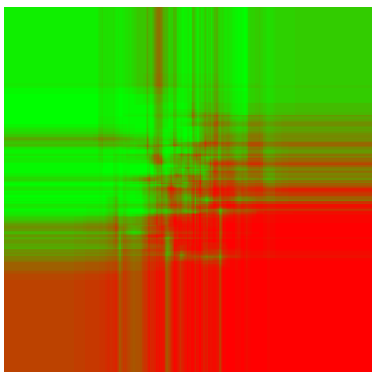
\includegraphics[width=\textwidth]{images/rf2.png}
        \caption{RF (50 Trees)}
    \end{subfigure}
    \begin{subfigure}[b]{0.3\textwidth}
        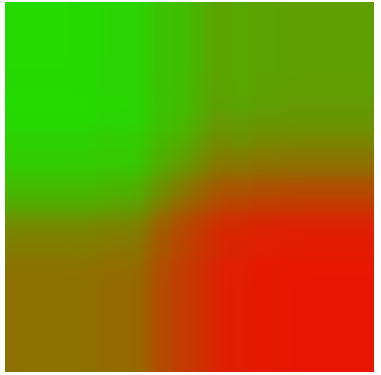
\includegraphics[width=\textwidth]{images/rf3.png}
        \caption{RF (2000 Trees)}
    \end{subfigure}
\end{figure}
\end{frame}

\begin{frame}{Out of bag samples}
\begin{center}
    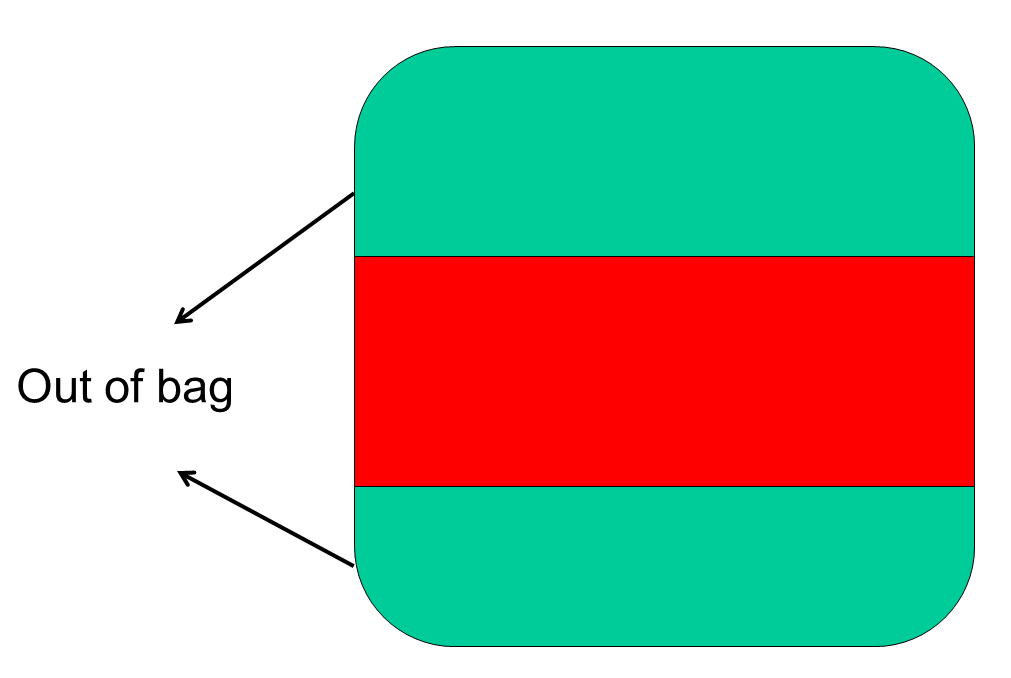
\includegraphics[scale=0.3]{images/outofbag.png}
\end{center}
\end{frame}

\begin{frame}{Random Forest \& overfitting}
\begin{center}
    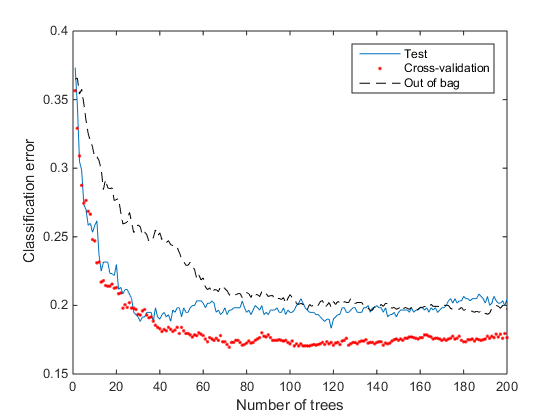
\includegraphics[scale=0.4]{images/rfcurves.png}
\end{center}
\begin{itemize}
    \item Не переобучается с ростом числа алгоритмов
\end{itemize}
\end{frame}

\begin{frame}{Feature impotance}
\begin{center}
    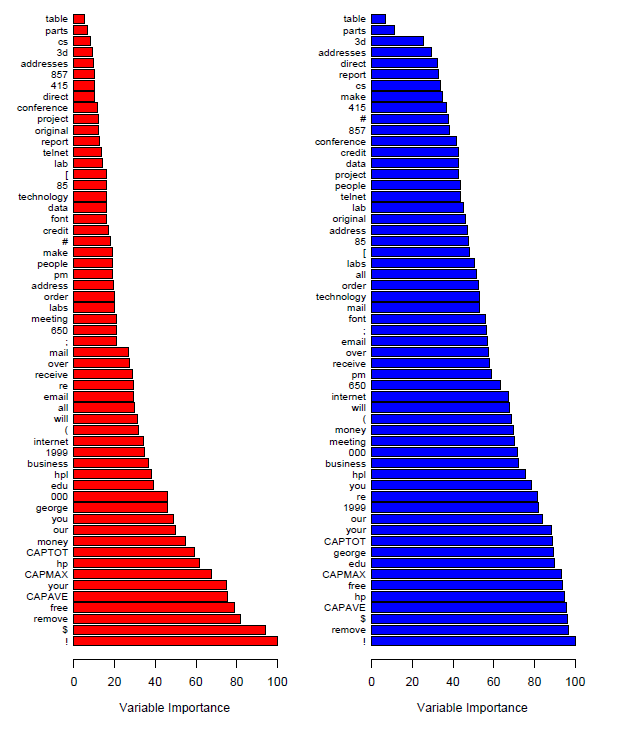
\includegraphics[scale=0.3]{images/impotance.png}
\end{center}
\end{frame}

\begin{frame}{Random Forest Clustering}
\begin{center}
    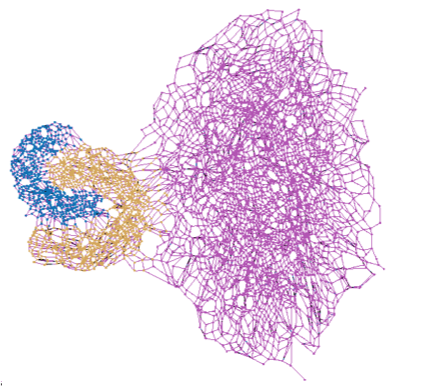
\includegraphics[scale=0.9]{images/RFCgraph.png}
\end{center}
\begin{block}{Концепция}
\end{block}
\begin{itemize}
    \item В один кластер попадают те примеры, которые чаще всего вместе попадали в
    листья деревьев
\end{itemize}
\end{frame}

\begin{frame}{Random Forest. Итоги}
\begin{itemize}
    \item[\color{green}\ding{52}] Алгоритм прост
    \item[\color{green}\ding{52}] Не пререобучается
    \item[\color{green}\ding{52}] Хорошо параллелится
    \item[\color{green}\ding{52}] Не требует сложной настройки параметров
    \item[\color{green}\ding{52}] Не требует нормализации данных (деревья решений)
    \item[\color{red}\ding{54}] Модели получаются большие и неинтерпретируемые
    \item[\color{red}\ding{54}] Плохо работает с полиномиальными зависимостями.
    \item[\color{red}\ding{54}] ``Медленно'' работает для большого объема данных.
\end{itemize}
\end{frame}

\begin{frame}{Extremely Randomized Trees}
\begin{center}
    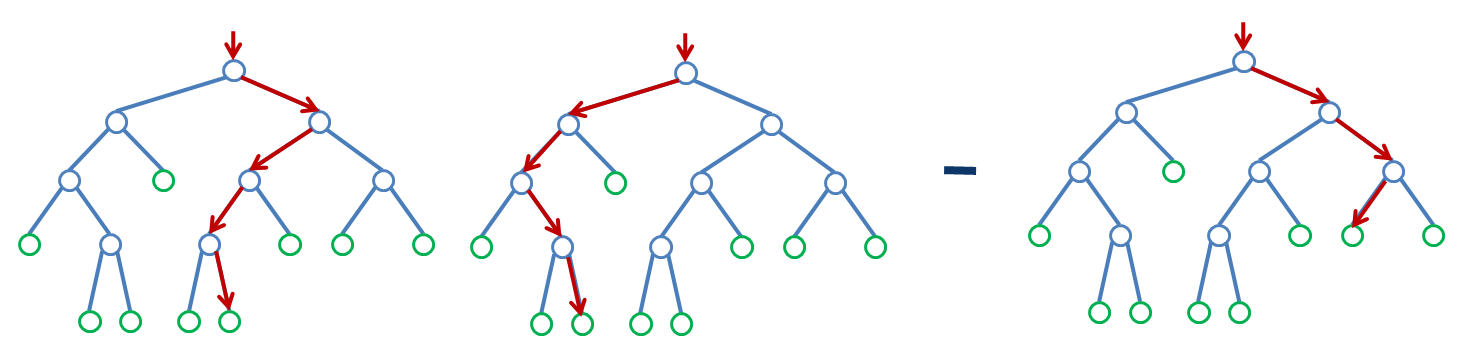
\includegraphics[scale=0.2]{images/ert.png}
\end{center}
\begin{itemize}
    \item Проверяем только один предикат на фичу
    \item Используем все фичи для каждого дерева
    \item \textcolor{red}{Работает в разы быстрее}
\end{itemize}
\end{frame}

\begin{frame}{Kaggle.com about Random Forest}
\begin{center}
    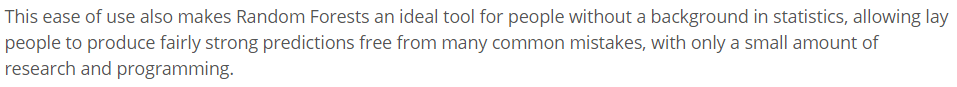
\includegraphics[scale=0.35]{images/kaggle.png}
\end{center}
\begin{itemize}
    \item \url{https://www.kaggle.com/wiki/RandomForests}
\end{itemize}
\end{frame}

\begin{frame}[fragile]{Задача}

{\bf Дано:} Имеется набор данных из системы поискового антиспама. \\
{\bf Требуется:} Требуется построить классификатор для представленных данных
на основе алгоритма Random Forest. Провести сравнение данного метода с
известными алгоритмами классификации. Ответить на вопросы.

\vspace{1em}
Пошаговая инструкция
\begin{enumerate}
    \item Скачать данные и запустить шаблон кода на python
    \url{http://goo.gl/gCQ7Y3}
\begin{shaded}
{\color{green} \begin{verbatim}
$ python rf.py -h
$ python rf.py -tr spam.train.txt -te spam.test.txt
\end{verbatim}}
\end{shaded}
    \item Сравнинить RF c другими известными алгоритмами классификации.
    \item Написать функцию подбирающую параметры числа деревьев и процента
    признаков в деревьях. Построить график.
    \item Ответить на вопрос: Почему качество классификации для класса spam выше
    чем для класса notspam?
\end{enumerate}

\end{frame}

\begin{frame}[plain]
\begin{center}
{\Large Вопросы}
\end{center}
\end{frame}

\end{document}
